% =====================================================================
% Owners: 2 (4.1-4.3), 4 (4.4)   Budget: ~1.4 pages incl. figure
% Source: slides 3-7, docs/architecture/*.md
% =====================================================================
\section*{4. System Design}

\begin{figure}[h]
\centering
% Owner 1: export slide 3 as PDF (crop) -> figures/architecture.pdf
\IfFileExists{figures/architecture.pdf}{%
  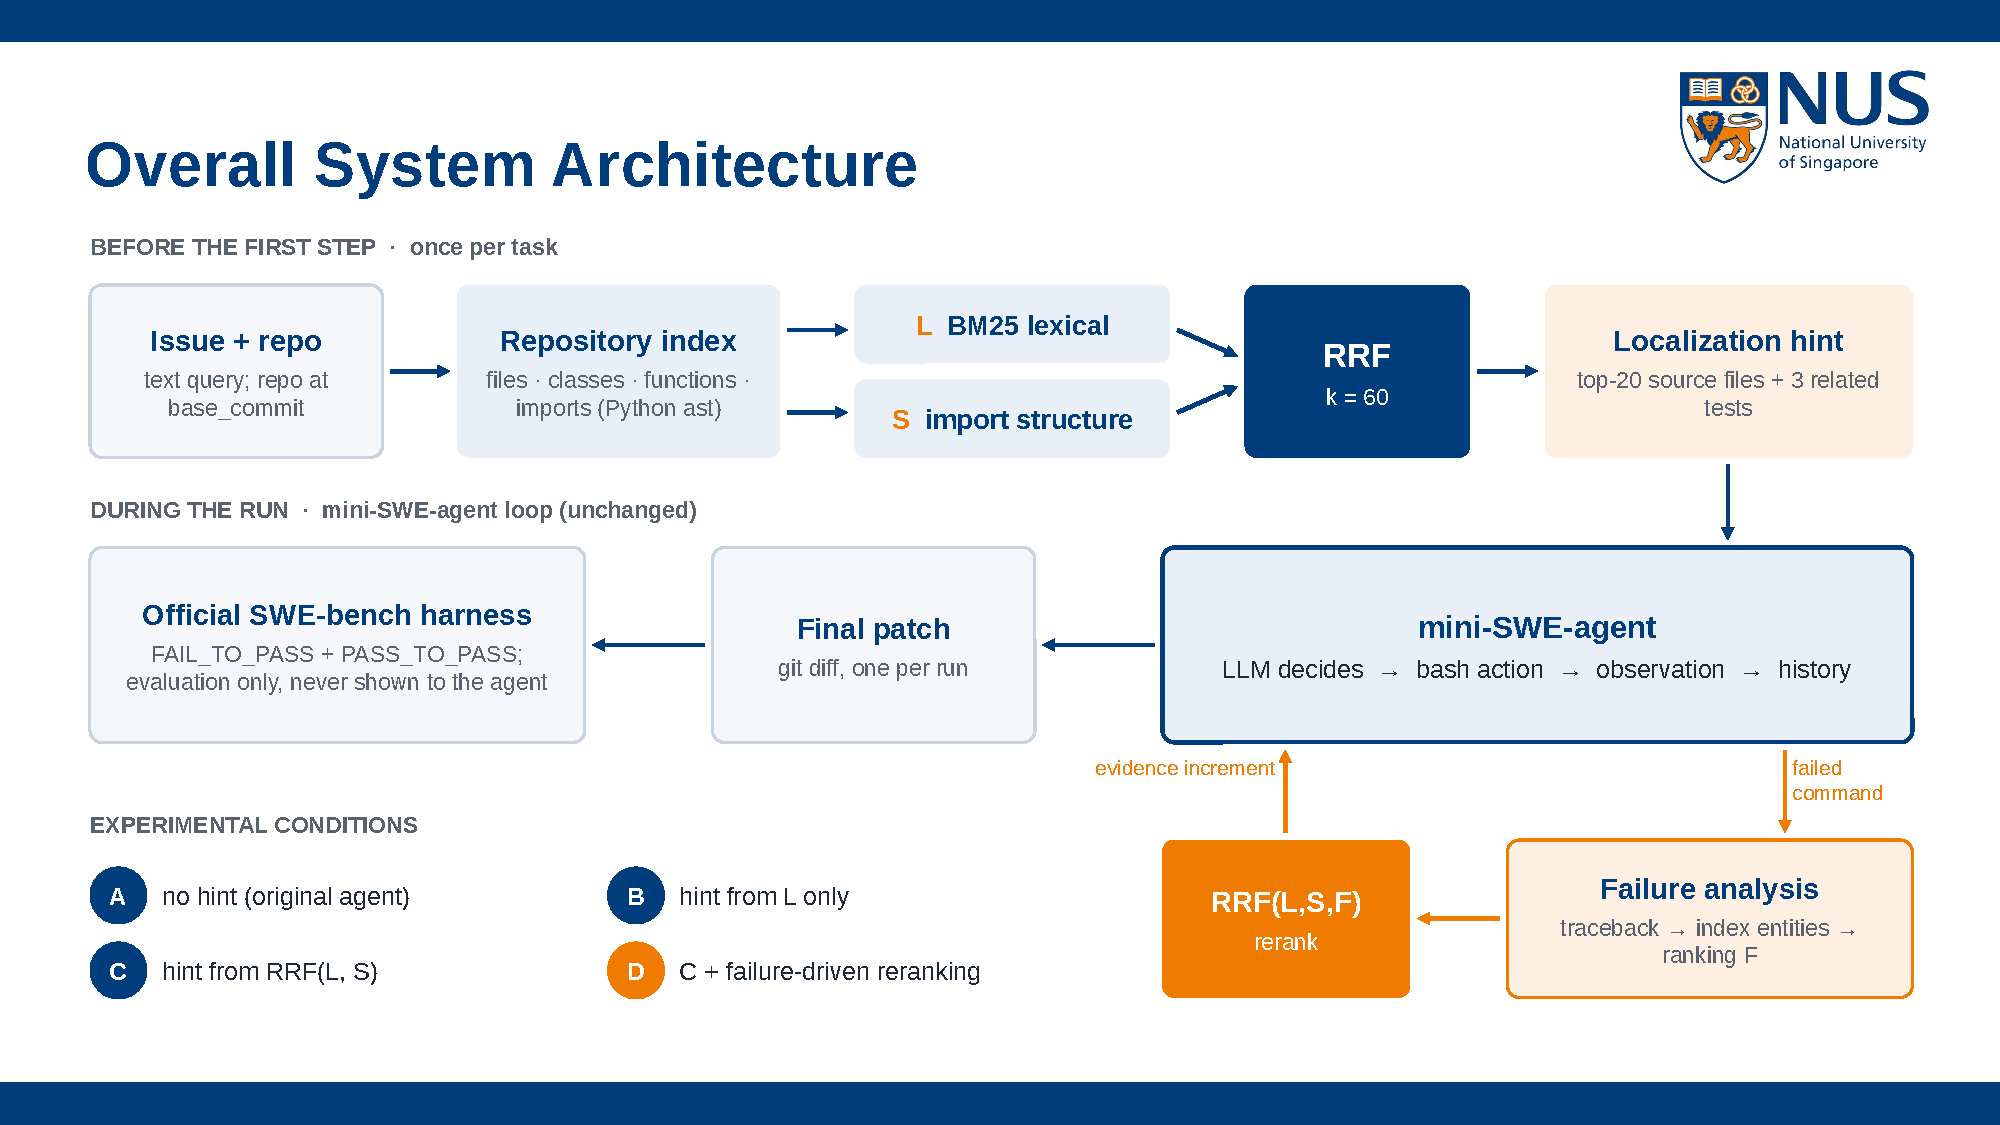
\includegraphics[width=\linewidth]{figures/architecture.pdf}%
}{%
  \fbox{\parbox[c][4.5cm][c]{0.9\linewidth}{\centering
  \todo{figures/architecture.pdf (export from slide 3)}}}%
}
\caption{System overview. The mini-SWE-agent loop is unchanged; \condB--\condD{} add a ranked
localization hint, and \condD{} reranks it when a failure yields usable evidence.}
\label{fig:arch}
\end{figure}

\subsection*{4.1 Repository index and lexical ranking}
% Owner 2. Implementation: src/repository/{ast_parser,indexer,swebench}.py, src/localization/keyword.py.
The index is the shared data layer for every condition. For each task we read every \texttt{.py}
file at the task's \texttt{base\_commit} directly from a git object store (no checkout), parse it
with Python's \texttt{ast} module, and store one record per module, class, function and method:
path, qualified symbol, line span, signature, docstring, and a retrieval text made of path, symbol
and source, truncated to 2,000 characters. Import statements are resolved to repository files,
giving each file $f$ a set of one-hop neighbours $N(f)$: the files it imports and the files that
import it. Files that fail to parse are recorded and skipped rather than aborting the build. On the
20 development tasks the index covers 27,484 files and 528,100 records; the only unparseable file
is a deliberate syntax-error fixture in Django's test suite. Building takes 0.4--13\,s per task and
is cached. In Condition~\condD{} the index is updated incrementally with the files the agent has
edited, so that traceback line numbers map to the right entities (Section~4.4).

The lexical ranking $L$ treats each record $e$ as a BM25 document~\cite{robertson2009bm25}, with
lower-cased identifier and number tokens, $k_1=1.5$ and $b=0.75$; the query is the issue text $q$.
A file takes the score of its best-matching entity,
\begin{equation*}
\mathrm{score}(e)=\sum_{t\in q}\mathrm{IDF}(t)\,
  \frac{\mathit{tf}_{t,e}\,(k_1+1)}{\mathit{tf}_{t,e}+k_1\bigl(1-b+b\,|e|/\mathit{avgdl}\bigr)},
\qquad
\mathrm{score}(f)=\max_{e\in f}\mathrm{score}(e),
\end{equation*}
so that one strongly matching function lifts its file while long files are not rewarded for
length alone. $L$ contains every file with a positive score (ties broken by path) and is the hint
source for Condition~\condB.

\subsection*{4.2 Structural ranking and RRF fusion}
% Owner 2. Implementation: src/localization/structural.py, src/localization/ranker.py.
The structural ranking $S$ uses the import graph to reach files the issue does not mention. The
seeds $Q$ are the top-10 files of $L$; each seed $q$ with lexical rank $r_L(q)$ shares a weight of
$1/r_L(q)$ equally among its non-test neighbours,
\begin{equation*}
s(f)=\sum_{q\in Q}\frac{\mathbf{1}[f\in N(q)]}{r_L(q)\,\max\bigl(1,|N(q)|\bigr)} .
\end{equation*}
$S$ lists the seeds first, in lexical order, followed by their neighbours in decreasing $s(f)$.
Condition~\condC{} fuses the two rankings with reciprocal rank fusion~\cite{cormack2009rrf},
$\mathrm{RRF}(f)=\sum_{r\in\{L,S\}}1/(60+r(f))$, where a file absent from a ranking contributes
nothing. RRF uses positions only, so BM25 scores and structural weights never need a common scale.

\paragraph{Design change from the proposal.} The proposal's $S$ contained only neighbours. In an
offline ablation on the development tasks (Appendix~A.2, Table~\ref{tab:dev-ablation}) that version
let files appearing in both lists overtake a correct file ranked first by BM25 alone
(django-11133: rank $1\to23$), lowering MRR from 0.500 to 0.393. Putting the seeds at the head of $S$
keeps $L$'s top~10 unchanged in $C$, so structure can only add files at ranks 11--20; this raised
Hit@20 from 0.75 to 0.85 with Hit@1, Hit@5 and MRR equal to or above $L$. The choice was made on
the development set before the held-out runs, so these numbers are optimistic; its effect on the
held-out tasks is reported in Section~5.1.

\subsection*{4.3 Prompt policy}
% Owner 2 (with 3). Implementation: src/agent/context.py (policy source_only+related_tests_v1).
In \condB--\condD{} the hint is appended once to the issue text before the first model call and is
labelled as navigation suggestions that the agent may ignore. It lists the top-20 \emph{source}
files of the condition's ranking, keeping their rank and score from the full ranking, and then, as
``possibly relevant existing tests'', the three highest-ranked test files of the same ranking
(an example is in Appendix~A.1). We adopted this policy after the development runs: most failures
there happened after the agent had already seen the right file, while test and documentation files
took on average 2.9 of the 20 slots. The source-file rule is the same one that defines the
evaluation targets (Section~5). The full, unfiltered ranking is logged for evaluation and is never
shown to the agent.

\subsection*{4.4 Failure-aware refinement (Condition D)}
% Owner 4. Source: slide 6. Wrap env.execute() and model.query().
% Pipeline: detect (exit status) -> parse (frames, exception, failing tests) -> map frames to index
% entities (index refreshed with edited files) -> rank F (nearest-to-exception first, 1/rank)
% -> RRF(L,S,F), w=1 -> short evidence note before next model call.
% Usability rules: >=1 frame maps to indexed source entity; setup errors never rerank;
% tests-only -> diagnostic note; stale workspace -> skipped; identical evidence not re-sent.
% Routing caps per run: rank_update 3, edit_recovery 2, diagnostic_only 1.
\todo{Failure-aware pipeline + usability rules (could be a 5-step list or pseudocode).}
